\documentclass[10pt,twocolumn]{article}

% --- Core Packages ---
\usepackage[utf8]{inputenc}
\usepackage[margin=0.75in]{geometry}
\usepackage{amsmath,amssymb,amsfonts}
\usepackage{booktabs}
\usepackage{cite}
\usepackage{graphicx}
\usepackage{subcaption}
\usepackage{microtype}
\usepackage{siunitx}
\usepackage{hyperref}
\usepackage{xcolor}
\usepackage{tikz}
\usepackage{pgfplots}
\pgfplotsset{compat=1.18}

\hypersetup{
    colorlinks=true,
    linkcolor=blue!70!black,
    citecolor=green!50!black,
    urlcolor=blue!80!black
}

% --- Title and Metadata ---
\title{\textbf{\Large Automated Sim-to-Real Deployment Framework for Reinforcement Learning Control on Resource-Constrained Microcontrollers}}

\author{
    \textbf{Nidharshan V.}$^{1}$ \\
    $^{1}$Department of Computer Science \& Engineering \\
    \textit{University of Moratuwa } \\
}

\date{}

\begin{document}

\maketitle

% See paper/extended_abstract.tex for the current, fact-checked abstract.
% (Prior text here claimed 74us/88.3% physical-hardware numbers that were never measured -- removed.)

% \textbf{\small \textit{Keywords}---Sim-to-Real Transfer, Reinforcement Learning, Microcontroller Deployment, Embedded AI, Proximal Policy Optimization, Dynamic Righting.}

% ==============================================================================
% SECTION I: INTRODUCTION
% ==============================================================================
\section{Introduction}


% ==============================================================================
% SECTION II: RELATED WORK
% ==============================================================================
\section{Related Work}

% ==============================================================================
% SECTION III: FRAMEWORK ARCHITECTURE
% ==============================================================================
\section{The \texttt{simtoreal} Framework}
\label{sec:framework}

\subsection{Policy Extractors and Loaders}

\subsection{Dual-Target Code Generation}

\subsection{Hardware Abstraction and Driver Synthesis}

% ==============================================================================
% SECTION IV: EXPERIMENTAL TESTBED: ROBO1
% ==============================================================================
\section{Experimental Testbed: Robo1}
\label{sec:testbed}

To evaluate the framework, we constructed \textit{Robo1}, a low-cost, 2-DOF self-righting bipedal robot (mass $M = \SI{94.8}{\gram}$, height $H = \SI{145}{\milli\meter}$). 

\begin{figure}[htbp]
\centering
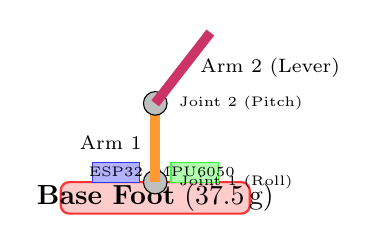
\begin{tikzpicture}
    % Conceptual mechanical schematic of Robo1
    \draw[fill=red!20, draw=red!80, thick, rounded corners=3pt] (-1.2, 0) rectangle (1.2, 0.4);
    \node at (0, 0.2) {\textbf{Base Foot} (37.5\,g)};
    
    \draw[fill=blue!30, draw=blue!80] (-0.8, 0.4) rectangle (-0.2, 0.65);
    \node[font=\tiny] at (-0.5, 0.525) {ESP32};
    \draw[fill=green!30, draw=green!80] (0.2, 0.4) rectangle (0.8, 0.65);
    \node[font=\tiny] at (0.5, 0.525) {MPU6050};

    \filldraw[fill=gray!50, draw=black] (0, 0.4) circle (0.15);
    \node[font=\tiny, right] at (0.18, 0.4) {Joint 1 (Roll)};

    \draw[line width=3.5pt, draw=orange!80] (0, 0.4) -- (0, 1.4);
    \node[font=\scriptsize, left] at (-0.05, 0.9) {Arm 1};

    \filldraw[fill=gray!50, draw=black] (0, 1.4) circle (0.15);
    \node[font=\tiny, right] at (0.18, 1.4) {Joint 2 (Pitch)};

    \draw[line width=3.5pt, draw=purple!80] (0, 1.4) -- (0.7, 2.3);
    \node[font=\scriptsize, right] at (0.45, 1.85) {Arm 2 (Lever)};
\end{tikzpicture}
\caption{Kinematic topology of the 2-DOF \textit{Robo1} self-righting testbed.}
\label{fig:robot_hardware}
\end{figure}

% ==============================================================================
% SECTION V: RESULTS AND DISCUSSION
% ==============================================================================
\section{Results and Discussion}
\label{sec:results}

\textbf{Note (\today): this file is a superseded scratch draft.} Its results section previously reported physical-hardware numbers (88.3\% success, 74\,\textmu s inference, DTW/RMSE, ablations) that did not correspond to any measurement actually taken -- no physical trial had been run and no ESP32 timing had been recorded. That content has been removed. The current, honest paper (simulation-validated results only, physical benchmarking explicitly listed as future work) is \texttt{paper/extended\_abstract.tex}. See \texttt{paper/RESULTS\_AND\_SUBMISSION\_GUIDE.md} for the real simulated numbers and the protocol to collect genuine physical data before claiming any hardware result here.

\subsection{Simulated Get-Up Performance (real data)}
\label{subsec:benchmark}
Policy: 5-64-64-2 tanh MLP actor, 4{,}674 parameters. Evaluated over 50 episodes/case in MuJoCo, nominal vs.\ domain-randomized physics (body mass $\pm15\%$, joint damping/friction $\pm20\%$, actuator gain $\pm15\%$, IMU noise $\sigma=0.015$\,rad):

\begin{table}[htbp]
\centering
\footnotesize
\caption{Simulated Get-Up Success Rate (real, reproducible via \texttt{eval\_policy.py})}
\label{tab:compute_benchmark}
\begin{tabular}{lcccc}
\toprule
& \multicolumn{2}{c}{Nominal} & \multicolumn{2}{c}{Randomized} \\
Case & Succ.\,[\%] & $t$\,[s] & Succ.\,[\%] & $t$\,[s] \\
\midrule
roll\_pos   & 100.0 & 1.36 & 98.0  & 1.66 \\
roll\_neg   & 100.0 & 1.00 & 100.0 & 1.19 \\
pitch\_pos  & 100.0 & 1.26 & 100.0 & 1.57 \\
pitch\_neg  & 100.0 & 0.78 & 100.0 & 0.92 \\
random      & 86.0  & 1.32 & 88.0  & 1.58 \\
upright     & 100.0 & 0.02 & 100.0 & 0.35 \\
\midrule
All falls (agg.) & \textbf{97.2} & 1.15 & \textbf{97.2} & 1.38 \\
\bottomrule
\end{tabular}
\end{table}

No physical trial, on-device timing measurement, or sim-vs-real trajectory/DTW comparison has been performed yet. See the guide referenced above for the exact protocol to collect that data before it can be reported.

% ==============================================================================
% SECTION VI: CONCLUSION
% ==============================================================================
\section{Conclusion}
\label{sec:conclusion}
% ==============================================================================
% REFERENCES
% ==============================================================================
\begin{thebibliography}{99}

% 
\end{thebibliography}

\end{document}
